\subsection[formulae]{Formulae}

\textit{Apply and justify properties of three-dimensional objects (e.g., the volume and surface area
formulas for prisms, pyramids, cones, cylinders, spheres)}

\subsubsection[formulae]{the volume and surface area formulas} 

\paragraph*{prisms}

A \textbf{prism} is a solid object with identical ends, flat faces, and the same cross section all along its length. The ends of a prism are $\parallel$ and each end is called a base. The side faces of a prism are parallelograms
(4-sided shapes with opposite sides parallel)

\vspace{2cm}


\vspace{2cm}
\subparagraph*{Surface Area} The surface area of a prism encompasses the surface area of both bases and all the faces.


\begin{figure}[h!]
    \begin{center}
        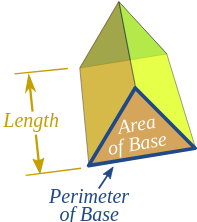
\includegraphics[scale=.45]{./public/images/prism-surface-area}
        \caption{Surface Area =  2 × Base Area
        + Base Perimeter × Length}
    \end{center}
\end{figure}

\subparagraph*{Volume} The Volume of a prism is the area of one end times the length of the prism:

$$V_{prism} = Base_{area} \times h$$

\paragraph{pyramids} A pyramid is made by connecting a base to an apex

\begin{figure}[h!]
    \begin{center}
        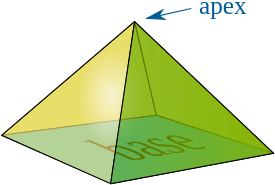
\includegraphics[scale=.45]{./public/images/pyramid}
        \caption{A pyramid is made by connecting a base to an apex}
    \end{center}
\end{figure}

\subparagraph*{pyramid volume}

$V_{pyramid} = \frac{1}{3} Base_{area} \times height $


\paragraph*{cones}


$$V_{cone} = \frac{1}{3} \pi r^2h$$


\paragraph*{cylinders} A \textit{cylinder} is not a polyhedron.A cylinder is like a prism with an infinite number of sides

\begin{figure}[h!]
    \begin{center}
        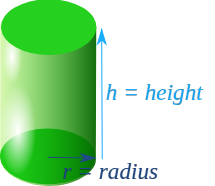
\includegraphics[scale=.45]{./public/images/cylinder}
        \caption{A pyramid is made by connecting a base to an apex}
    \end{center}
\end{figure}

\subparagraph*{volume of a cylinder} $V_{cylinder} = \pi r^2h$

\paragraph{spheres} Of all the shapes, a sphere has the smallest surface area for a volume.

\begin{figure}[h!]
    \begin{center}
        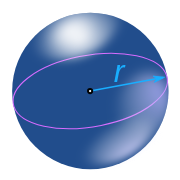
\includegraphics[scale=.25]{./public/images/sphere}
        \caption{Of all the shapes, a sphere has the smallest surface area for a volume.}
    \end{center}
\end{figure}

\subparagraph*{volume of a sphere} $V_{sphere} = \frac{4}{3} \pi r^3$